\documentclass[10pt,journal]{IEEEtran}
\usepackage{xcolor,soul,framed}
\usepackage[cmex10]{amsmath}
\usepackage{changepage}
\usepackage{setspace}
\usepackage{booktabs}
\usepackage{fancyhdr}
\usepackage{longtable}
\usepackage{blindtext}
\usepackage{scrextend}
\usepackage{csquotes}
\usepackage{lipsum}  
\usepackage{enumitem}
\usepackage{multicol}
\usepackage{multirow}
\usepackage{graphicx}
\graphicspath{{./figs/},{./AuthorBio/}}
\usepackage{array}
\usepackage{mdwmath}
\usepackage{mdwtab}
\usepackage{eqparbox}
\usepackage{url}
\usepackage{threeparttable}
\usepackage{algorithmic}
\usepackage{textcomp}
\usepackage{amssymb,amsfonts}
\usepackage[sort&compress,numbers]{natbib}

\bibliographystyle{IEEEtran}
\usepackage{stfloats} 

\renewenvironment{description}[1][1pt]
{\list{}{\labelwidth=0pt \leftmargin=#1 \let\makelabel\descriptionlabel}}
{\endlist}

\begin{document}
\bstctlcite{IEEEexample:BSTcontrol}

\title{Hardware-efficient emulation of leaky integrate-and-fire model using template-scaling-based exponential function approximation}

\author{Jeeson~Kim, Vladimir~Kornijcuk, ChangMin~Ye, Doo~Seok~Jeong,
\thanks{J.~Kim, V.~Kornijcuk, C.~Ye and D. S.~Jeong are with Division of Materials Science and Engineering, Hanyang University, 222 Wangsimni-ro, Seongdong-gu, Seoul 04763, South Korea.\protect\\ E-mail: dooseokj@hanyang.ac.kr}}

\markboth{IEEE TRANSACTION ON CIRCUITS AND SYSTEMS I: REGULAR PAPERS,~Vol.~X, No.~X, X~2020}
{Author \MakeLowercase{\textit{et al.}}: Journal title}

\maketitle
\begin{abstract}
We present a method to emulate a leaky integrate-and-fire (LIF) model in a field-programmable gate array (FPGA) in a hardware-efficient manner. The simplified spike-response model (SRM$_\textrm{0}$) is chosen as an LIF model. For the hardware-efficient implementation of SRM$_\textrm{0}$, we adopt the template-scaling-based exponential function approximation (TS-EFA). This method allows high-precision and low-latency exponential function approximations with the efficient use of hardware resources. We subsequently propose an algorithm for SRM$_\textrm{0}$, which leverages the advantages of the TS-EFA method. An implementation of 512 neurons conforming to SRM$_\textrm{0}$ in an FPGA highlights (i) high-precision of SRM$_\textrm{0}$ emulation (average error rate: $<2\%$ compared with simulations using real-valued variables and parameters), (ii) low latency (eight clock cycles), and (iii) high-efficiency in hardware usage (only 125b memory per neuron).
\end{abstract}

\begin{IEEEkeywords}
Leaky integrate-and-fire model, spike-response model, template-scaling-based exponential function approximation, spiking neural network
\end{IEEEkeywords}


\IEEEpeerreviewmaketitle
\section{Introduction}
\IEEEPARstart{T}{he} main advantage of spiking neural networks (SNNs) is its expressive capability in both static and dynamic domains \cite{jeong2018tutorial,pfeiffer2018deep, tavanaei2019deep,roy2019towards}. 
For reproducing their dynamic behaviors, different spiking neuron models, e.g., Stein’s model \cite{stein1965theoretical}, Hodgkin-Huxley model \cite{izhikevich2003simple}, and spike-response model (SRM) \cite{gerstner2002spiking}, have been proposed. 
Available spiking neuron models are diverse, but commonly involve temporal kernels that are given by exponential functions \cite{gerstner2002spiking,dayan2001theoretical}.
Hardware implementations of spiking neurons can provide several benefits, including real-time and low-power operations \cite{indiveri2011neuromorphic}.
Nevertheless, considering a large-scale implementation, calculating the exponential functions for all neurons can result in significant workload on hardware. 
To address this heavy workload, our work proposes an efficient implementation of the simplified SRM (SRM$_\textrm{0}$) as a leaky integrate-and-fire (LIF) model in a memory-centric architecture. The implementation uses a newly proposed exponential function approximation (EFA) method that aims at high-accuracy and high-efficiency in hardware usage. The architecture is memory-centric because the EFA method is based on lookup tables (LUTs). The exponential functions in the model are approximated by repeatedly scaling a segment of pre-calculated exponential functions (template). 
This method is therefore referred to as the template-scaling-based EFA (TS-EFA) \cite{kim2020isqed}.

Section \ref{sec:tsefa} elaborates an implementation of TS-EFA. 
Section~\ref{sec:impl_LIF} is dedicated to the implementation of SRM$_\textrm{0}$ using TS-EFA modules and its performance compared with several relevant works.
Section~\ref{sec:con} concludes our work.


\section{Template-scaling-based exponential function approximation}
\label{sec:tsefa}

\subsection{Template-scaling method}\label{subsec:ts}
TS-EFA  uses a template-scaling method to approximate exponential relaxation functions at high precision.
In this method, a set of pre-calculated exponential function values in a specific time range is used as a template. The template is repeatedly scaled to calculate the function values over the entire input range. 
Knowing $y_1$ = exp(-$t_1$$\mathbin{/}$$\tau$) for $t_1$ within the time range of a template, $y_2$ (= exp(-$t_2$$\mathbin{/}$$\tau$)) for $t_2$ out of the template range equals $y_2$ = exp(-($t_2$-$t_1$)$\mathbin{/}$$\tau$)$\cdot$exp(-$t_1$$\mathbin{/}$$\tau$) = \textit{S}$\cdot$$y_1$. 
Therefore, by introducing the scaling factor \textit{S}, any exponential function values in the entire time range (0 \textendash~$t_\textrm{max}$) can be approximated. 
The entire time range is divided into multiple bins of the same width ($w_\textrm{bin}$) of which the first bin (BIN\textunderscore0) is taken as the template (Fig.~\ref{fig:fig1}). 

%%%%%%%%%%%%%%%%%%%%%%%%%%%%
\begin{figure}[tb]\centering
    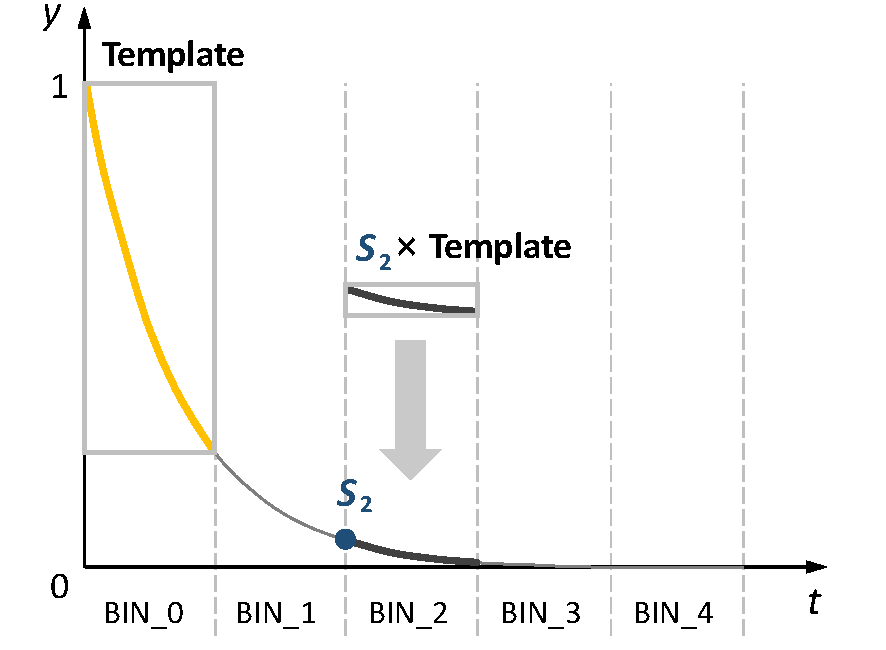
\includegraphics[width=3.1in]{fig1}
    \caption{\label{fig:fig1} Illustration of an exponential relaxation function approximation using the template-scaling method.}
\end{figure}
%%%%%%%%%%%%%%%%%%%%%%%%%%%%

The implementation of TS-EFA requires two LUTs, namely TEMP\textunderscore LUT and SCAL\textunderscore LUT (template LUT and scaling LUT, respectively). 
The LUT length can be optimized to ensure the high accuracy of the approximation while maintaining the memory-efficiency of TS-EFA. 
To begin, we define the relationship between the length of TEMP\textunderscore LUT ($l_\textrm{tpl}$), bin width ($w_\textrm{bin}$), and sampling precision ($\Delta t$). 
TEMP\textunderscore LUT stores the pre-calculated function values in the first bin (template). 
Thus, the length is determined by the bin width ($w_\textrm{bin}$) and sampling precision ($\Delta t$):
%%%%%%%%%%%%%%%%%%%%%%%%%%%%%%%%
\begin{equation}\label{equ:equ1}
    l_{\textrm{tpl}}=w_{\textrm{bin}}\mathbin{/}\Delta t.
\end{equation}
%%%%%%%%%%%%%%%%%%%%%%%%%%%%%%%%
Because SCAL\textunderscore LUT stores the first function value in each bin, the length of SCAL\textunderscore LUT equals the number of bins in the entire time range (0 \textendash~$t_\textrm{max}$):
%%%%%%%%%%%%%%%%%%%%%%%%%%%%%%%%
\begin{equation}\label{equ:equ2}
    l_{\textrm{scl}}=t_{\textrm{max}}\mathbin{/}w_{\textrm{bin}}.	
\end{equation}
%%%%%%%%%%%%%%%%%%%%%%%%%%%%%%%%
Here, the maximum time $t_\textrm{max}$ should be sufficiently large for the exponential function value to attain the minimum value with binary encoding bits ($b$), leading to the optimal condition, exp(-$t_\textrm{max}$$\mathbin{/}$$\tau$) = $2^{\textrm{-}b}$. 
The length $l_\textrm{scl}$ can be defined by plugging this equation into equation  \eqref{equ:equ2}, resulting in
%%%%%%%%%%%%%%%%%%%%%%%%%%%%%%%%
\begin{equation}\label{equ:equ3}
    l_\textrm{scl} = b \cdot \tau \cdot \ln2 \mathbin{/} w_\textrm{bin}.	
\end{equation}
%%%%%%%%%%%%%%%%%%%%%%%%%%%%%%%%
The total memory \textit{M} dedicated to TEMP\textunderscore LUT and SCAL\textunderscore LUT in a $b$-bit format is therefore expressed as
%%%%%%%%%%%%%%%%%%%%%%%%%%%%%%%%
\begin{equation}\label{equ:equ4}
    M=b\cdot w_{\textrm{bin}}\mathbin{/}\Delta t + b^2 \cdot\tau\cdot \ln2\mathbin{/}w_\textrm{bin}. 
\end{equation}
%%%%%%%%%%%%%%%%%%%%%%%%%%%%%%%%
The optimal $w_\textrm{bin}$ in terms of memory usage can be evaluated by solving the equation $d\textit{M}$$\mathbin{/}$$dw_\textrm{bin}$ = 0 for $w_\textrm{bin}$, leading to the optimal bin width $w_\textrm{bin0}$,
%%%%%%%%%%%%%%%%%%%%%%%%%%%%%%%%
\begin{equation}\label{equ:equ5}
    w_\textrm{bin0} = \sqrt{\Delta t\cdot b\cdot\tau\cdot \ln2}.	
\end{equation}
%%%%%%%%%%%%%%%%%%%%%%%%%%%%%%%%
The optimal length of TEMP\textunderscore LUT and SCAL\textunderscore LUT ($l_\textrm{tmp0}$ and $l_\textrm{scl0}$) can be obtained by entering equation \eqref{equ:equ5} into \eqref{equ:equ1} and \eqref{equ:equ2}, yielding
%%%%%%%%%%%%%%%%%%%%%%%%%%%%%%%%
\begin{equation}\label{equ:equ6}
    l_\textrm{tpl0} = l_\textrm{scl0} 
    = w_\textrm{bin0}\mathbin{/}\Delta t 
    = \sqrt{b\cdot \tau \cdot \ln2 \mathbin{/}\Delta t}.
\end{equation}
%%%%%%%%%%%%%%%%%%%%%%%%%%%%%%%%
Because the lengths $l_\textrm{tmp0}$ and $l_{\textrm{scl0}}$ are integers, the term $w_\textrm{bin0}$$\mathbin{/}$$\Delta t$ needs to be integerized using a round-up operator ceil($\cdot$). 
Therefore, the optimal bin width $w_\textrm{opt,bin0}$ can be obtained as
%%%%%%%%%%%%%%%%%%%%%%%%%%%%%%%%
\begin{equation}\label{equ:equ7}
    w_\textrm{opt,bin0} = \textrm{ceil}(w_\textrm{bin0}\mathbin{/}\Delta t) \cdot \Delta t.	
\end{equation}
%%%%%%%%%%%%%%%%%%%%%%%%%%%%%%%%
Fig. \ref{fig:fig2} illustrates an example of TS-EFA with the optimal memory usage for $b$ = 16, $\Delta t$ = 0.5, and $\tau$ = 1.

%%%%%%%%%%%%%%%%%%%%%%%%%%%%
\begin{figure}[tbh]\centering
    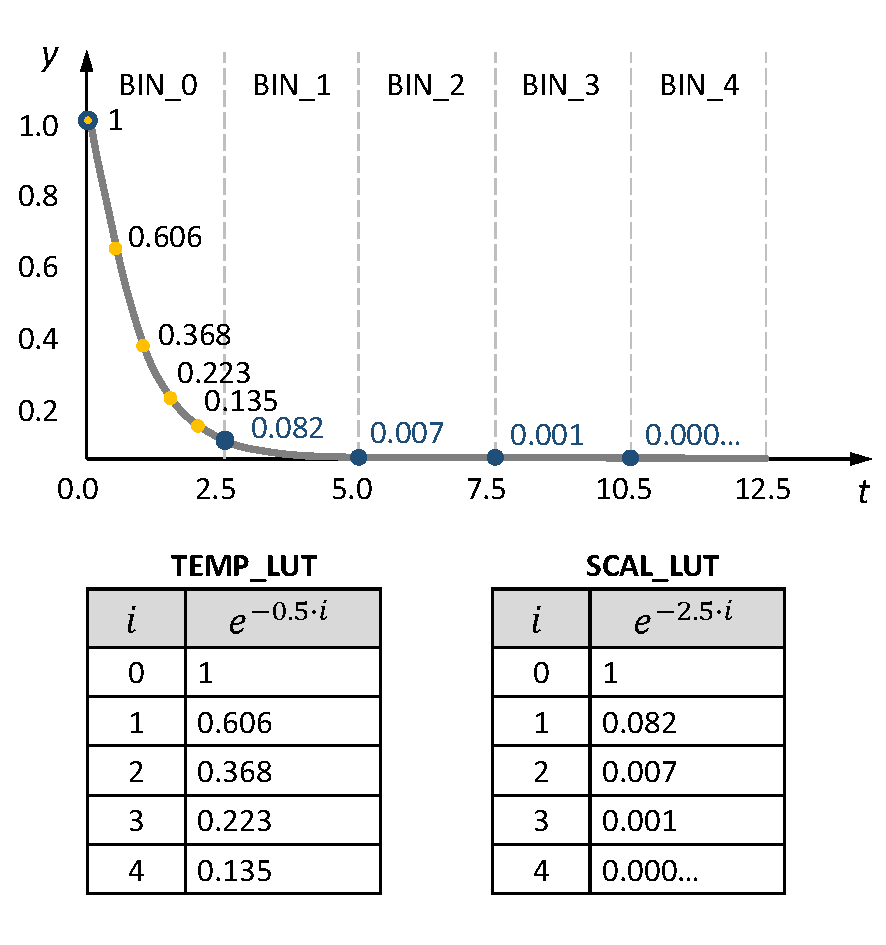
\includegraphics[width=3.3in]{fig2}
    \caption{\label{fig:fig2} Exponential function encoding using TEMP\textunderscore LUT and SCAL\textunderscore LUT ($b$ = 16, $\tau$ = 1, $\Delta t$ = 0.5).}
\end{figure}
%%%%%%%%%%%%%%%%%%%%%%%%%%%%

%%%%%%%%%%%%%%%%%%%%%%%%%%%%
\begin{figure*}[tbh]\centering
    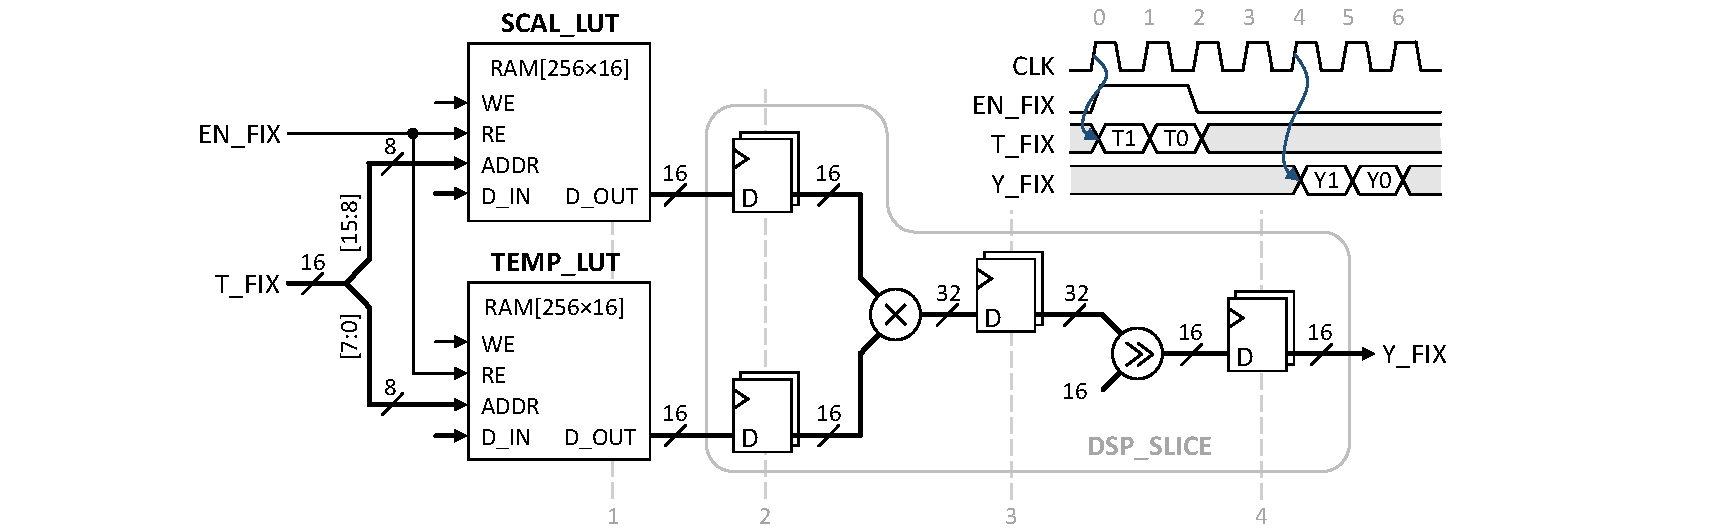
\includegraphics[width=7.1in]{fig3}
    \caption{\label{fig:fig3} RTL and timing diagrams of the EXP\textunderscore FIX module.} 
\end{figure*}
%%%%%%%%%%%%%%%%%%%%%%%%%%%%

\subsection{Implementation of TS-EFA modules} \label{subsec:tsefa_imp}
We implemented a fixed time constant-based EFA (EXP\textunderscore FIX) module, approximating \textit{f}($t_\textrm{f}$) = exp(-$t_\textrm{f}$$\cdot$$\Delta t_\textrm{f}$$\mathbin{/}$$\tau_\textrm{f}$), where $t_\textrm{f}$, $\Delta t_\textrm{f}$, and $\tau_\textrm{f}$ denote the index of a given time step, sampling precision, and fixed time constant, respectively. 
Fig. \ref{fig:fig3} shows a register-transfer level (RTL) diagram of the EXP\textunderscore FIX module.
The EXP\textunderscore FIX module uses a 256$\times$16 random access memory (RAM) block for each of TEMP\textunderscore LUT and SCAL\textunderscore LUT.
The LUTs are pre-organized using the aforementioned memory-optimization procedure and filled with values for a pre-defined time constant $\tau_\textrm{f}$. 
The LUTs can be read using a read enable signal (EN\textunderscore FIX) and index signal (T\textunderscore FIX). 
The T\textunderscore FIX signal indicates the index of a given time step ($t_\textrm{f}$) in a 16-bit integer format. 
T\textunderscore FIX is separated into two 8-bit signals (T\textunderscore FIX[8:15] and T\textunderscore FIX[0:7]), which are used as address pointers for TEMP\textunderscore LUT and SCAL\textunderscore LUT, respectively. 
The values retrieved from the LUTs are multiplied to produce a 32-bit fixed-point value. 
This value is rounded to a 16-bit fixed-point value using the right shift operator, eventually yielding the approximation result Y\textunderscore FIX. 
In this EXP\textunderscore FIX implementation, we use one built-in DSP slice for both multiplication and right-shift operations by fully-pipelining. 
Consequently, the module takes four clock cycles to output Y\textunderscore FIX (timing diagram in Fig. \ref{fig:fig3}). 

%%%%%%%%%%%%%%%%%%%%%%%%%%%%%%
\begin{figure*}[bh]\centering
    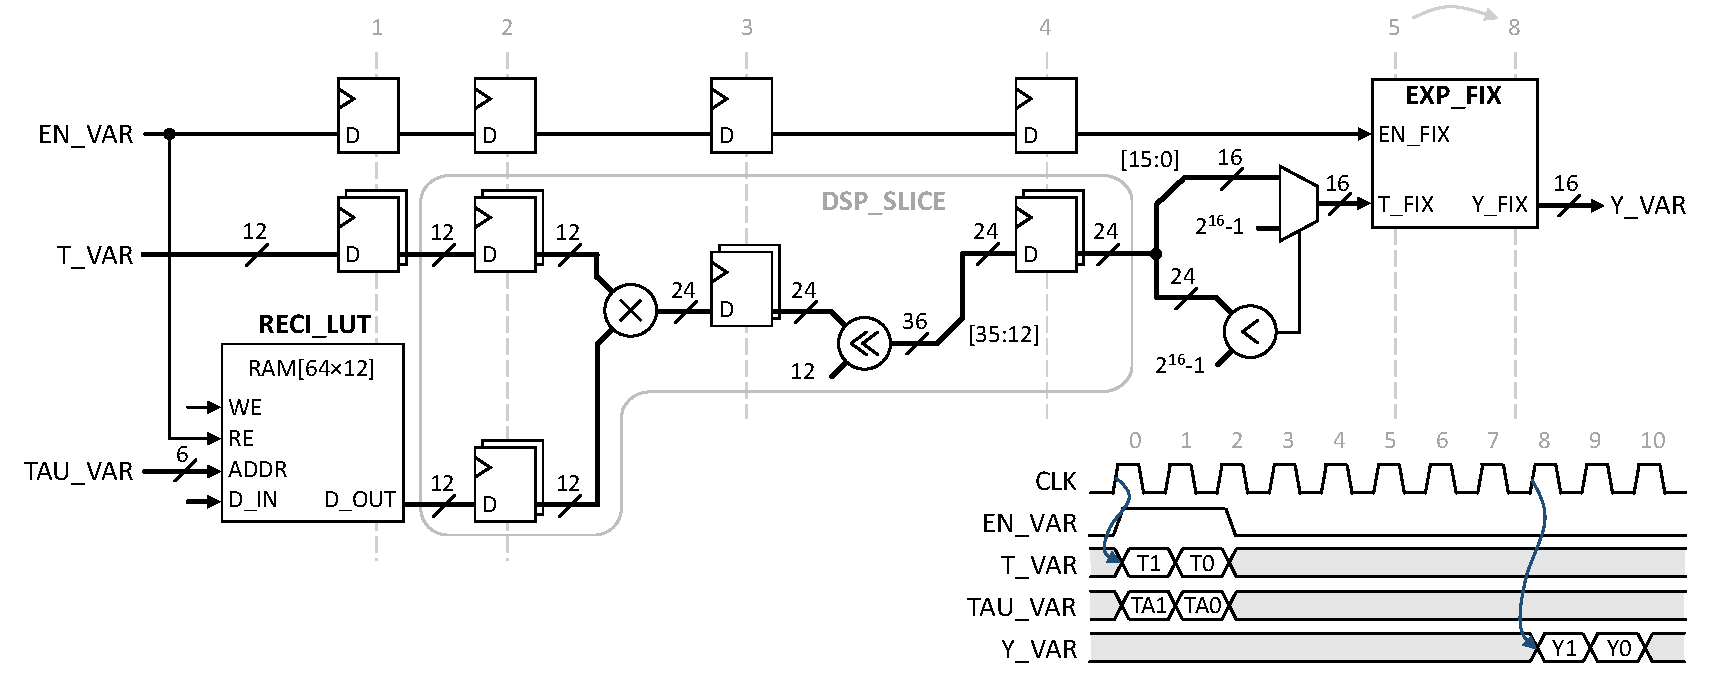
\includegraphics[width=7.1in]{fig4}
    \caption{\label{fig:fig4} RTL and timing diagrams of the EXP\textunderscore VAR module.} 
\end{figure*}
%%%%%%%%%%%%%%%%%%%%%%%%%%%%%%

Generally, the exponential kernels in SNNs use multiple time constants. 
Nevertheless, the EXP\textunderscore FIX module can be utilized as a function approximator with an additional circuit that effectively converts the time constant of the EXP\textunderscore FIX module into a desired one. 
Let us consider a function \textit{f}($t_\textrm{var}$) = exp(-$t_\textrm{var}$$\cdot$$\Delta t_\textrm{var}$$\mathbin{/}$$\tau_\textrm{var}$), which is to be approximated using the EXP\textunderscore FIX module for a kernel \textit{f}($t_\textrm{f}$) = exp(-$t_\textrm{f}$$\cdot$$\Delta t_\textrm{f}$$\mathbin{/}$$\tau_\textrm{f}$) with $\tau_\textrm{f}$~=~1.
Equating these two equations results in
%%%%%%%%%%%%%%%%%%%%%%%%%%%%%%
\begin{equation}\label{equ:equ8}
    t_\textrm{f} = t_\textrm{var} \cdot \Big(\frac{\Delta t_\textrm{var}}{\tau_\textrm{var}}\Big) \cdot \Big(\frac{1}{\Delta t_\textrm{f}}\Big).
\end{equation}
%%%%%%%%%%%%%%%%%%%%%%%%%%%%%%
We implemented a TS-EFA module that leaves the time constant as a variable, referred to as a EXP\textunderscore VAR module (Fig. \ref{fig:fig4}).
This module features simultaneous implementations of multiple functions with multiple time constants using a single EXP\textunderscore FIX module. 
The EXP\textunderscore VAR module requires an additional LUT (RECI\textunderscore LUT) to store 64 different $\Delta t_\textrm{var}$$\mathbin{/}$$\tau_\textrm{var}$ values, each in a 12-bit fixed-point format. 
Note that all 12 bits are dedicated to a fractional part because $\Delta t_\textrm{var}$$\mathbin{/}$$\tau_\textrm{var}<1$.

The T\textunderscore VAR and TAU\textunderscore VAR signals input a time step index $t_{\textrm{var}}$ (12-bit integer) and chosen $\Delta t_\textrm{var}$$\mathbin{/}$$\tau_\textrm{var}$ value, respectively.
As depicted in Fig. \ref{fig:fig4}, a chosen $\Delta t_\textrm{var}$$\mathbin{/}$$\tau_\textrm{var}$ value is retrieved from RECI\textunderscore LUT during the first clock cycle, and the multiplication $t_\textrm{var}$$\cdot$\big($\frac{\Delta  t_\textrm{var}}{\tau_\textrm{var}}$\big) in Equation \eqref{equ:equ8} is performed during the second clock cycle.
The multiplication yields a 24-bit fixed-point value, consisting of a 12-bit integer and 12-bit fractional part. 
By setting the time step $\Delta t_\textrm{f}$ to $2^{\textrm{-}p}$ (here, $p$~=~12), the last multiplication in Equation \eqref{equ:equ8} is performed by using a left-shift operator during the third clock cycle. 
Further, the fractional part of the result is removed because the EXP\textunderscore FIX module accepts only integer inputs, yielding 24-bit $t_\textrm{f}$.
The multiplication and left-shift operation are performed using only one built-in DSP slice by fully-pipelining. 

Because the EXP\textunderscore FIX accepts 16-bit integer inputs, the upper bound of 24-bit $t_\textrm{f}$ is set to 2$^\textrm{16}$-1 ($t_\textrm{max}$).
With the EXP\textunderscore FIX module ($\tau_\textrm{f} = 1$, $b$ = 16, and $\Delta t_\textrm{f}$ = 2$^\textrm{-12}$), setting $t_\textrm{max}$ to 2$^\textrm{16}$-1 ensures the full relaxation of the function \textit{f}($t_\textrm{f}$) = exp(-$t_\textrm{f}$$\cdot$$\Delta t_\textrm{f}$$\mathbin{/}$$\tau_\textrm{f}$) because \textit{f}(2$^\textrm{16}$-1) $\ll$ 2$^{\textrm{-}b}$ for $\tau_\textrm{f}$~=~1. 
Therefore, when $t_\textrm{f}$ exceeds 2$^\textrm{16}$-1, the index $t_\textrm{f}$ becomes stuck to 2$^\textrm{16}$-1.
This process is conducted during the fourth clock cycle as depicted in Fig. \ref{fig:fig4}.
Otherwise, the index $t_\textrm{f}$ is input to the EXP\textunderscore FIX module, and the module outputs a 16-bit fixed-point value (Y\textunderscore VAR) in four clock cycles.
Therefore, it takes eight clock cycles in aggregate for the EXP\textunderscore VAR module to approximate an exponential function on a given time step (timing diagram in Fig. \ref{fig:fig4}).

%%%%%%%%%%%%%%%%%%%%%%%%%%%
\begin{table*}[tbh]\centering
\caption{\label{tab:tab1} Performance comparison of TS-EFA with related works}
\renewcommand{\arraystretch}{1.25} 
\begin{threeparttable}\small
\begin{tabular}[ht]{p{1.78cm}p{1.57cm}p{1.64cm}p{1.6cm}p{1.6cm}p{1.47cm}p{1.48cm} p{1.6cm}p{1.6cm}} \toprule \toprule
    &\multirow{3}{1.57cm}{\textbf{Wielgosz\\\textit{et al}. \cite{wielgosz2008highly}}\\} 
    &\multirow{3}{1.64cm}{\textbf{de Dinechin \\and Pasca \\\cite{de2010floating}}} 
    &\multirow{3}{1.6cm}{\textbf{Malík \cite{malik2015high}} \\~\\~} 
    &\multirow{3}{1.6cm}{\textbf{Ortega-\\Zamorano\\\cite{ortega2014high}}} 
    &\multirow{3}{1.47cm}{\textbf{Nilsson\\\textit{et al}. \cite{nilsson2014hardware}}\\} 
    &\multirow{3}{1.48cm}{\textbf{Partzsch\\\textit{et al}. \cite{partzsch2017fixed}}\\}
    &\multicolumn{2}{c}{\multirow{2}{3.2cm}{~~~~~~~~\textbf{This work}}} \\
    &&&&&&&\multirow{2}{1.6cm}{\textbf{EXP\textunderscore FIX}} &\multirow{2}{1.6cm}{\textbf{EXP\textunderscore VAR}}\\  
    &&&&&&&\\ \midrule
    \multirow{2}{1.73cm}{\textbf{Platform}\\\textbf{(Technology)}} 
        &\multirow{2}{1.57cm}{\hfil Virtex-4\\\hfil FPGA} 
        &\multirow{2}{1.64cm}{\hfil Virtex-5\\\hfil FPGA} 
        &\multirow{2}{1.6cm}{\hfil Virtex-4\\\hfil FPGA} 
        &\multirow{2}{1.6cm}{\hfil Virtex-5\\\hfil FPGA} 
        &\multirow{2}{1.47cm}{\hfil ASIC\\\hfil (65~nm)}   
        &\multirow{2}{1.48cm}{\hfil ASIC\\\hfil (28~nm)}
        &\multicolumn{2}{c}{\multirow{2}{3.2cm}{\hfil Virtex-7 FPGA \\}}\\
    &&&&&&&&\\
    \multirow{2}{1.73cm}{\textbf{Method}\\} 
        &\multirow{2}{1.57cm}{\hfil Polynomial\\\hfil approx.} 
        &\multirow{2}{1.64cm}{\hfil Polynomial\\\hfil approx.} 
        &\multirow{2}{1.6cm}{\hfil Power\\\hfil series}    
        &\multirow{2}{1.6cm}{\hfil Linear\\interpolation} 
        &\multirow{2}{1.47cm}{\hfil Taylor\\\hfil series} 
        &\multirow{2}{1.48cm}{\hfil Polynomial\\\hfil approx.} 
        &\multicolumn{2}{c}{\multirow{2}{3.2cm}{\hfil Template scaling\\}}\\
    &&&&&&&&\\
    \multirow{2}{1.73cm}{\textbf{Data format (Precision)}} 
        &\multirow{2}{1.57cm}{Floating-pnt \\\hfil (Double)} 
        &\multirow{2}{1.64cm}{Floating-pnt \\\hfil (Double)} 
        &\multirow{2}{1.6cm}{Floating-pnt \\\hfil (Single)} 
        &\multirow{2}{1.6cm}{\hfil Fixed-pnt\\} 
        &\multirow{2}{1.47cm}{\hfil Fixed-pnt\\} 
        &\multirow{2}{1.48cm}{\hfil Fixed-pnt\\}
        &\multicolumn{2}{c}{\multirow{2}{3.2cm}{~~~~~~~Fixed-pnt\\}}\\
    &&&&&&&&\\
    \multirow{2}{1.73cm}{\textbf{Clock speed}\\\textbf{[MHz]}} 
        &\multirow{2}{1.57cm}{\hfil 200\\} 
        &\multirow{2}{1.64cm}{\hfil 119\textendash310\\} 
        &\multirow{2}{1.6cm}{\hfil 65\textendash66\\}
        &\multirow{2}{1.6cm}{\hfil 868\\}
        &\multirow{2}{1.47cm}{\hfil 25\\}
        &\multirow{2}{1.48cm}{\hfil 500\\} 
        &\multicolumn{2}{c}{\multirow{2}{3.2cm}{~~~~~~~~~~~500\\}}\\
    &&&&&&&&\\
    \multirow{2}{1.78cm}{\textbf{Latency}\\\textbf{[Clock cycle]}} 
        &\multirow{2}{1.57cm}{\hfil 30\\} 
        &\multirow{2}{1.64cm}{\hfil 12\textendash35\\}
        &\multirow{2}{1.6cm}{\hfil 11\textendash15\\} 
        &\multirow{2}{1.6cm}{\hfil 2\\} 
        &\multirow{2}{1.47cm}{\hfil $<$2\\}
        &\multirow{2}{1.48cm}{\hfil 6\\} 
        &\multirow{2}{1.6cm}{~~~~~~4\\} 
        &\multirow{2}{1.6cm}{~~~~~8\\}\\
    &&&&&&&\\
    \multirow{2}{1.73cm}{\textbf{LUTs as logic}}
        &\multirow{2}{1.57cm}{\hfil 13,614\\} 
        &\multirow{2}{1.64cm}{1,601\textendash1,867\\} 
        &\multirow{2}{1.6cm}{2,498\textendash2,559\\} 
        &\multirow{2}{1.6cm}{\hfil 78\\} 
        &\multirow{2}{1.47cm}{\hfil \textendash\\} 
        &\multirow{2}{1.48cm}{\hfil \textendash\\} 
        &\multirow{2}{1.6cm}{~~~~~74\\} 
        &\multirow{2}{1.6cm}{~~~~~76\\}\\
    &&&&&&&\\
    \multirow{2}{1.73cm}{\textbf{DSP slice}} 
        &\multirow{2}{1.57cm}{\hfil 0} 
        &\multirow{2}{1.64cm}{\hfil 12} 
        &\multirow{2}{1.6cm}{\hfil 0} 
        &\multirow{2}{1.6cm}{\hfil 1} 
        &\multirow{2}{1.47cm}{\hfil \textendash} 
        &\multirow{2}{1.48cm}{\hfil \textendash} 
        &\multirow{2}{1.6cm}{~~~~~~1} 
        &\multirow{2}{1.6cm}{~~~~~2}\\
    &&&&&&&\\
    \multirow{2}{1.73cm}{\textbf{Memory}\\} 
        &\multirow{2}{1.57cm}{\hfil 29$\times$18Kb \\\hfil BRAM$^\dagger$} 
        &\multirow{2}{1.64cm}{\hfil 5$\times18$Kb \\\hfil BRAM$^\dagger$} 
        &\multirow{2}{1.6cm}{\hfil N/A\\} 
        &\multirow{2}{1.6cm}{\hfil 924$\times$64b \\\hfil Dist. RAM$^\ddagger$} 
        &\multirow{2}{1.47cm}{\hfil N/A\\} 
        &\multirow{2}{1.48cm}{\hfil 404Bytes\\}
        &\multirow{2}{1.6cm}{~176$\times$64b\\Dist. RAM$^\ddagger$} 
        &\multirow{2}{1.6cm}{~16$\times$64b\\Dist. RAM$^\ddagger$}\\
    &&&&&&&&\\
    \multirow{2}{1.73cm}{\textbf{Error\\ (Type)}} 
        &\multirow{2}{1.57cm}{\hfil $<$1 ulp\\}
        &\multirow{2}{1.64cm}{\hfil $<$1 ulp\\} 
        &\multirow{2}{1.6cm}{\hfil 3.0$\times$10$^\textrm{-6}$ \\(Max. abs.)}
        &\multirow{2}{1.6cm}{\hfil 2.0$\times$10$^\textrm{-4}$ \\(Max. abs.)}
        &\multirow{2}{1.47cm}{\hfil 5.4$\times$10$^\textrm{-6}$ \\(Max. abs.)} 
        &\multirow{2}{1.48cm}{\hfil 3.0$\times$10$^\textrm{-5}$ \\(Max. abs.)} &\multicolumn{2}{c}{\multirow{2}{3.2cm}{~~~~~~~~~2.1$\times$10$^\textrm{-5}$ \\~~~~~~~(Max. abs.)}}\\
    &&&&&&&&\\\bottomrule \bottomrule
\end{tabular}
\begin{tablenotes}\small
\item[$\dagger$]: Block RAM
\item[$\ddagger$]: Distributed RAM
\end{tablenotes}
\end{threeparttable}
\end{table*}
%%%%%%%%%%%%%%%%%%%%%%%%%%%%

\subsection{Performance of template-scaling-based exponential function approximation}
\label{subsec:tsefa_per}
The EXP\textunderscore FIX and EXP\textunderscore VAR modules were implemented in a Virtex-7 field-programmable gate array (FPGA) at 500 MHz clock speed.
The modules were analyzed in terms of hardware consumption and approximation accuracy. 
The results are compared with related works in Table \ref{tab:tab1}. 
\cite{wielgosz2008highly} implemented a polynomial-based EFA using a double-precision floating-point format in a Virtex-4 FPGA, highlighting a high approximation accuracy---less than one unit in the last place (ulp). 
However, this implementation requires large hardware resources and large pipeline latency (30 clock cycles) at 200 MHz clock speed. 
Similarly, \cite{de2010floating} proposed a polynomial-based EFA using a double-precision floating-point format in a Virtex-5 FPGA, but considerably reduced hardware consumption and pipeline latency compared with \cite{wielgosz2008highly}.
This method uses DSP slices instead of several LUTs (as logic) to reduce memory usage. 
\cite{malik2015high} proposed a power series-based EFA using a single-precision floating-point data format in a Virtex-4 FPGA. 
This implementation highlights excellent approximation accuracy (maximum absolute error 3$\times$10$^\textrm{-6}$) and low pipeline latency. 
However, challenges are heavy hardware consumption (2,498 \textendash~2,559 LUTs) and low operation speed (65 \textendash~66 MHz). 
\cite{ortega2014high} prototyped an EFA in a Virtex-5 FPGA using a linear interpolation method with a fixed-point format.
It features high operation speed ($>$800 MHz), low latency (two clock cycles), and a few LUTs in use. 
Nevertheless, a high error rate (2$\times$10$^\textrm{-4}$) and significant memory usage are notable shortcomings. 
The application-specific integrated circuit (ASIC)-based works in \cite{nilsson2014hardware} and \cite{partzsch2017fixed} realized EFA solutions using a Taylor series approximation and polynomial-based approximation, respectively. 
The ASIC solution to the EFA in a fixed-point format indicates a considerable improvement on approximation accuracy compared with \cite{ortega2014high} that also used a fixed-point format. 

The EXP\textunderscore FIX module highlights low hardware consumption: 74 LUTs as logic, one DSP slice, and 176 distributed RAMs (each 64-bit) in aggregate. 
The improvement in efficiency in hardware usage is significant compared with the other FPGA-based EFA implementations  \cite{wielgosz2008highly,de2010floating,malik2015high,ortega2014high}.
The EXP\textunderscore FIX features low latency (only four clock cycles) at 500 MHz. 
The EXP\textunderscore VAR module needs an additional DSP slice and one additional LUT. 
It is also noteworthy that the EXP\textunderscore VAR module uses only 16 distributed RAMs (each 64-bit) compared with the EXP\textunderscore FIX module using 176 distributed RAMs (each 64-bit). 
The reduction is because the submodule EXP\textunderscore FIX in the EXP\textunderscore VAR module uses a read-only memory for TEMP\textunderscore LUT and SCAL\textunderscore LUT instead of RAMs.
TS-EFA also highlights high approximation accuracy (maximum absolute error of approximately 2.1$\times10^\textrm{-5}$) (Fig. \ref{fig:fig5}).

%%%%%%%%%%%%%%%%%%%%%%%%%%%%%%
\begin{figure}[bh]\centering
    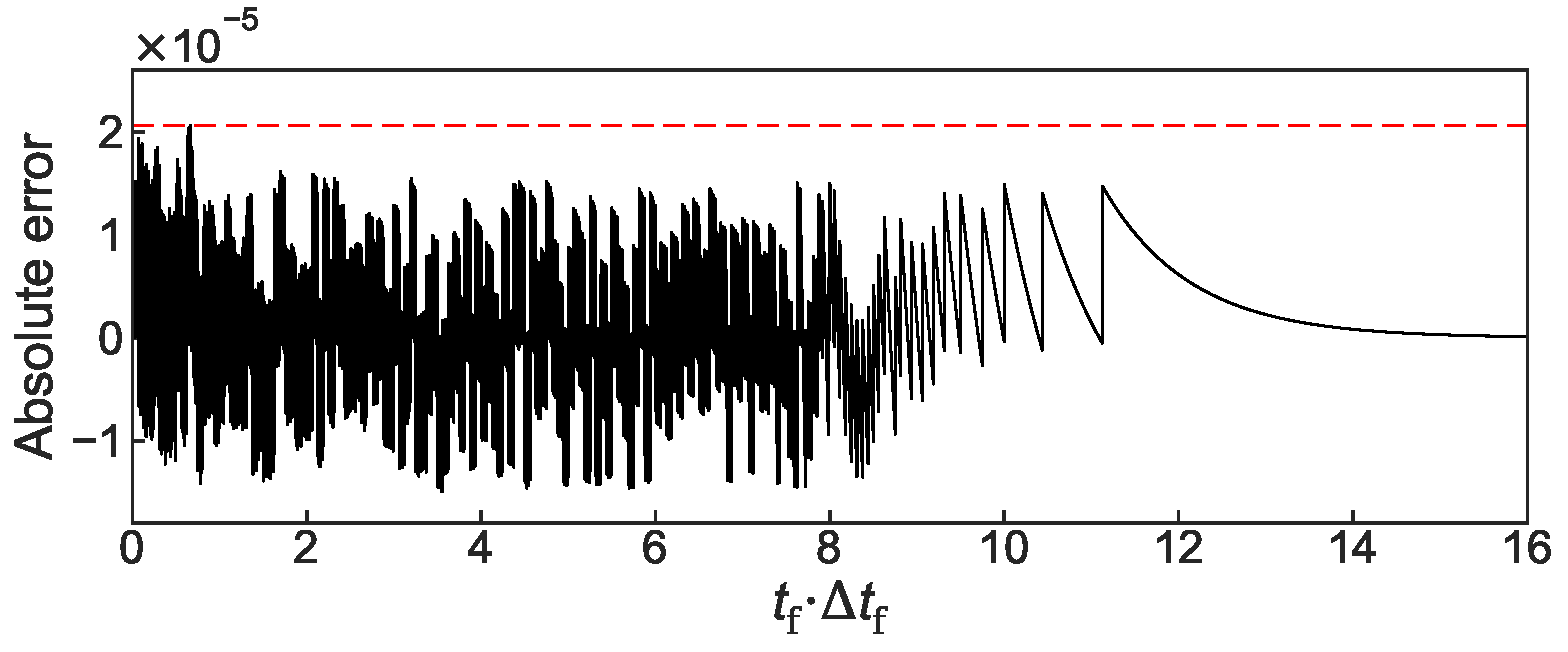
\includegraphics[width=3.4in]{fig5}
    \caption{\label{fig:fig5} Absolute error in EFAs using the EXP\textunderscore FIX module ($\tau_\textrm{f}$ = 1).}
\end{figure}
%%%%%%%%%%%%%%%%%%%%%%%%%%%%%%
%This value is obtained by measuring the difference between the EFA values and the calculation result using the real-value. The evaluation time range is between 0 to 16, with a sampling step size $\Delta$\textit{t}~=~$2^{-12}$ and a time constant $\tau$~=~1.


\section{Implementation of leaky integrate-and-fire model}\label{sec:impl_LIF}

\subsection{Leaky integrate-and-fire model}
The LIF neuron model is simple but sufficiently rich in dynamics for temporal coding \cite{gerstner2002spiking}. 
The model includes only two internal variables (synaptic current and membrane potential) to describe spiking behavior in response to input spikes (a.k.a. presynaptic spikes). 
When Neuron $i$ receives a presynaptic spike train from Neuron $j$, the spike train $\rho_j$ is modeled as 
$\rho_j$~=~$\sum_f\delta$\big($t$ - $t_j^{\textrm{(}f\textrm{)}}$\big); where $t_j^{\textrm{(}f\textrm{)}}$ denotes the timing of the $f$th spike in the spike train from Neuron $j$. 
This spike train is input to Neuron $i$ through a synapse $w_{ij}$, evoking synaptic current $i_\textrm{syn}$---a low-pass filtered version of input spikes in the LIF neuron model as follows.
%%%%%%%%%%%%%%%%%%%%%%%%%%%%%%
\begin{equation}\label{equ:equ9}
    i_\textrm{syn}(t) = \big[k_\textrm{s} \ast \rho_j \big](t),		
\end{equation}
%%%%%%%%%%%%%%%%%%%%%%%%%%%%%%
where the synaptic current kernel $k_\textrm{s}$ with a time constant $\tau_\textrm{s}$ and synaptic weight $w_{ij}$ is given by 
%%%%%%%%%%%%%%%%%%%%%%%%%%%%%%
\begin{equation}\label{equ:equ10}
    k_\textrm{s} = \frac{w_{ij}}{\tau_\textrm{s}} e^{-t\mathbin{/}\tau_\textrm{s}}.		
\end{equation}
%%%%%%%%%%%%%%%%%%%%%%%%%%%%%%
The membrane potential $u_\textrm{m}$ is subsequently evaluated by integrating the following equation with membrane resistance \textit{R}.
%%%%%%%%%%%%%%%%%%%%%%%%%%%%%%
\begin{equation}\label{equ:equ11}
    \tau_\textrm{m}\frac{du_\textrm{m}}{dt}=-u_\textrm{m}+i_\textrm{syn}\textit{R},	
\end{equation}
%%%%%%%%%%%%%%%%%%%%%%%%%%%%%%
where $\tau_\textrm{m}$ denotes the time constant of a membrane potential decay. 
The time-dependent membrane potential can be calculated by solving \eqref{equ:equ11} with \eqref{equ:equ9} numerically.
Nevertheless, the integration is expensive, particularly, when addressing large-scale networks.

%%%%%%%%%%%%%%%%%%%%%%%%%%%%%
\begin{table}[b]\centering
\begin{threeparttable}\small
\begin{tabular}[ht]{p{8.4cm}}\toprule
    \textbf{Algorithm 1:} Updation of membrane potential $u_\textrm{m}$, and auxiliary functions ($u_\textrm{1}$, $u_\textrm{2}$, $u_\textrm{3}$) on a given time step \\\midrule
    \textbf{Input:} Input spike $\delta_j$ (=0 when no input spike, and 1 otherwise) and $u_\textrm{1}$, $u_\textrm{2}$, $u_\textrm{3}$ on the previous time step \\
    \textbf{Output:} Output spike $\delta_i$ (=0 when no output spike, 1 otherwise) and $u_\textrm{m}$, $u_\textrm{1}$, $u_\textrm{2}$, $u_\textrm{3}$ on the current time step\\ \midrule

    Evaluate $u_\textrm{m}$, $u_\textrm{1}$, $u_\textrm{2}$, $u_\textrm{3}$ on time step $t$:\\
    $u_\textrm{1}$[$t$] $\leftarrow$ $u_\textrm{1}$[$t$-1]$\cdot$exp(-$\Delta t$$\mathbin{/}$$\tau_\textrm{m}$) + $\tau_\textrm{m}$$\cdot$$w_{ij}$$\cdot$($\tau_\textrm{m}$ - $\tau_\textrm{s}$)$^\textrm{-1}$$\cdot$$\delta_j$\\
    $u_\textrm{2}$[$t$] $\leftarrow$ $u_\textrm{2}$[$t$-1]$\cdot$exp(-$\Delta t$$\mathbin{/}$$\tau_\textrm{s}$) + $\tau_\textrm{m}$$\cdot$$w_{ij}$$\cdot$($\tau_\textrm{m}$ - $\tau_\textrm{s}$)$^\textrm{-1}$$\cdot$$\delta_j$\\
    $u_\textrm{3}$[$t$] $\leftarrow$ $u_\textrm{3}$[$t$-1]$\cdot$exp(-$\Delta t$$\mathbin{/}$$\tau_\textrm{m}$)\\
    
    $u_\textrm{m}$[$t$] $\leftarrow$ ($u_\textrm{1}$[$t$] - $u_\textrm{2}$[$t$]) - $u_\textrm{3}$[$t$]\\
    $\delta_i\leftarrow$ 0\\
    
    \textbf{if} $u_\textrm{m}$[$t$]$\geq$$u_\textrm{th}$ \textbf{then}\\
        ~~~$\delta_i\leftarrow$ 1\\
        ~~~$u_\textrm{1}$[$t$]~$\leftarrow$ 0\\
        ~~~$u_\textrm{2}$[$t$]~$\leftarrow$ 0\\
        ~~~$u_\textrm{3}$[$t$]~$\leftarrow u_\textrm{hyp}$\\
\textbf{end if}\\\bottomrule
\end{tabular}
\end{threeparttable}
\end{table} 
%%%%%%%%%%%%%%%%%%%%%%%%%%%%%


SRM$_\textrm{0}$ \cite{gerstner2002spiking} offers a workaround solution to \eqref{equ:equ11}, which converts \eqref{equ:equ11} into a convolution of an exponential function-based kernel $\epsilon$ and input spike train $\rho_j$. 
The model also considers a refractory period using a convolution of an exponential function-based kernel $\eta$ and output spike train $\rho_i$.
The membrane potential $u_\textrm{m}$ in the SRM$_\textrm{0}$ is therefore given by
%%%%%%%%%%%%%%%%%%%%%%%%%%%%%%
\begin{equation}\label{equ:equ12}
    u_\textrm{m}(t) = w_{ij}[\epsilon\ast\rho_{j}](t)+[\eta \ast\rho_i](t),
\end{equation}
%%%%%%%%%%%%%%%%%%%%%%%%%%%%%%
where 
%%%%%%%%%%%%%%%%%%%%%%%%%%%%%%
\begin{equation}\label{equ:equ13}
    \epsilon(t) =\frac{\tau_\textrm{m}}{\tau_\textrm{m}-\tau_\textrm{s}} \big(e^{-t\mathbin{/}\tau_\textrm{m}}- e^{-t\mathbin{/}\tau_\textrm{s}}\big) \Theta(t),
\end{equation}
%%%%%%%%%%%%%%%%%%%%%%%%%%%%%%
and 
%%%%%%%%%%%%%%%%%%%%%%%%%%%%%%
\begin{equation}\label{equ:equ14}
    \eta(t)=\Big[u_\textrm{hyp}-u_\textrm{m} \Big(t_i\Big)\Big] e^{-t\mathbin{/}\tau_\textrm{m}}\Theta(t).
\end{equation}
%%%%%%%%%%%%%%%%%%%%%%%%%%%%%%
The Heaviside step function is denoted by $\Theta$($t$).
Here, the resting membrane potential is set to 0~V, and the hyperpolarized membrane potential $u_\textrm{hyp}$ is negative. 
When the membrane potential exceeds a threshold for spiking ($u_\textrm{th}$), an output spike is elicited at $t_i$.  
The pre-exponential factor in \eqref{equ:equ14} includes $u_\textrm{m}$($t_i$) that indicates the membrane potential immediately before the spike timing $t_i$.
Therefore, the membrane potential attains the hyperpolarized potential $u_\textrm{hyp}$ immediately after output spike generation at $t_i$.

SRM$_\textrm{0}$ involves two exponential sub-kernels in the kernel $\epsilon$ in \eqref{equ:equ13}.
%%%%%%%%%%%%%%%%%%%%%%%%%%%%%%
\begin{equation}\label{equ:equ15}
   \epsilon_1 =\frac{\tau_\textrm{m}}{\tau_\textrm{m}-\tau_\textrm{s}} e^{-t\mathbin{/}\tau_\textrm{m}}\Theta(t),
\end{equation}
%%%%%%%%%%%%%%%%%%%%%%%%%%%%%%
and 
%%%%%%%%%%%%%%%%%%%%%%%%%%%%%%
\begin{equation}\label{equ:equ16}
   \epsilon_2 = \frac{\tau_\textrm{m}}{\tau_\textrm{m}-\tau_\textrm{s}} e^{-t\mathbin{/}\tau_\textrm{s}}\Theta(t),
\end{equation}
%%%%%%%%%%%%%%%%%%%%%%%%%%%%%%
We separately consider three sub-functions ($u_\textrm{1}$, $u_\textrm{2}$, and $u_\textrm{3}$; $u_\textrm{m}$ = $u_\textrm{1}$ - $u_\textrm{2}$ - $u_\textrm{3}$) for the three kernels in \eqref{equ:equ13} and \eqref{equ:equ14}, which are given by
%%%%%%%%%%%%%%%%%%%%%%%%%%%%%%
\begin{equation}\label{equ:equ17}
    u_1(t)=w_{ij}[\epsilon_1 \ast \rho_j ](t),
\end{equation}
%%%%%%%%%%%%%%%%%%%%%%%%%%%%%%
\begin{equation}\label{equ:equ18}
    u_2(t)=w_{ij}[\epsilon_2 \ast \rho_j ](t),
\end{equation}
%%%%%%%%%%%%%%%%%%%%%%%%%%%%%%
and
%%%%%%%%%%%%%%%%%%%%%%%%%%%%%%
\begin{equation}\label{equ:equ19}
    u_3(t)=[\eta \ast \rho_i](t).
\end{equation}
%%%%%%%%%%%%%%%%%%%%%%%%%%%%%%
SRM$_\textrm{0}$ is capable of membrane potential evaluation by simply updating these auxiliary functions ($u_\textrm{1}$, $u_\textrm{2}$, and $u_\textrm{3}$) on every time step. 
The detailed algorithm is presented in pseudocode in Algorithm 1.

\subsection{Implementation in FPGA}
Algorithm 1 was modified to be Algorithm 2 for its efficient implementation in an FPGA using the TS-EFA method. 
The modifications are as follows.

\begin{itemize}
    \item The auxiliary functions $u_\textrm{1}$, $u_\textrm{2}$, and $u_\textrm{3}$ in Algorithm 1 are normalized to the absolute value of hyperpolarized membrane potential $\mathrm{\lvert}$$u_\textrm{hyp}$$\mathrm{\lvert}$, referred to as U1, U2, and U3, respectively. Likewise, the threshold for spiking $u_\textrm{th}$ is normalized, referred to as UTH0. In this way, the pre-exponential factor for U3 is fixed to one so that one multiplication for U3 evaluation can be avoided.
    \item Pre-exponential factor PRE1 and exponential function Y\textunderscore FIX1 are separately considered (Instruction 1) and subsequently multiplied to evaluate the auxiliary function U1 (Instruction 2) unlike Algorithm 1. The same holds for the auxiliary function U2. However, for the auxiliary function U3, the multiplication is unnecessary because of the aforementioned normalization (Instruction 4).
    \item We introduce a new membrane potential UM0 that is determined by U1 and U2 only (Instruction 3). The refractory function U3 effectively alters the spiking threshold instead. That is, Instruction 5 compares UM0 with UTH0+U3 rather than UM0-U3 with UTH0. In this way, we save one-bit (sign) for each U3 value. 
\end{itemize}

%%%%%%%%%%%%%%%%%%%%%%%%%%%%%
\begin{table}[tb]\centering
\begin{threeparttable}\small
\begin{tabular}[ht]{p{8.4cm}}\toprule
    {\textbf{Algorithm 2:} Updation of effective membrane potential UM0 and auxiliary functions (U1, U2, U3) on a given time step}\\ \midrule
    {\textbf{Input:} Input spike SP\textunderscore IN (=0 when no input spike, and 1 otherwise), timing of the last input spike $\hat{t_j}$, and U1 and U2 on the previous time step} \\
    {\textbf{Output:} Output spike SP\textunderscore OUT (=0 when no output spike, and 1 otherwise), timing of the last output spike $\hat{t_i}$, and UM0, U1, U2, and U3 on the current time step}\\ \midrule
    
    Evaluate $u_\textrm{m}$, $u_\textrm{1}$, $u_\textrm{2}$, $u_\textrm{3}$ on time step $t$:\\
    $\hat{t_j}$ $\leftarrow$ $\hat{t_j}$ + ($t$ - $\hat{t_j}$)$\cdot$SP\textunderscore IN\\
    PRE1 $\leftarrow$ (U1[$t$-1] + $\tau_\textrm{m}$$\cdot$[($\tau_\textrm{m}$ - $\tau_\textrm{s}$)$\cdot$$\mathrm{\lvert}$$u_\textrm{hyp}$$\mathrm{\lvert}$]$^\textrm{-1}$$\cdot$$w_{ij}$)$\cdot$SP\textunderscore IN
    + PRE1$\cdot$(1-SP\textunderscore IN)   //Instruction 1\\ 
    U1[$t$] $\leftarrow$ PRE1$\cdot$Y\textunderscore FIX1[$t$-$\hat{t_j}$] //Instruction 2\\
    PRE2 $\leftarrow$ (U2[$t$-1] + $\tau_\textrm{m}$$\cdot$[($\tau_\textrm{m}$ - $\tau_\textrm{s}$)$\cdot$$\mathrm{\lvert}$$u_\textrm{hyp}$$\mathrm{\lvert}$]$^\textrm{-1}$$\cdot$$w_{ij}$)$\cdot$SP\textunderscore IN 
    + PRE2$\cdot$(1-SP\textunderscore IN)\\
    U2[$t$] $\leftarrow$ PRE2$\cdot$Y\textunderscore FIX2[$t$-$\hat{t_j}$]\\
    UM0[$t$] $\leftarrow$ U1[$t$] - U2[$t$] //Instruction 3\\
    U3[$t$] $\leftarrow$ Y\textunderscore FIX3[$t$-$\hat{t_i}$] //Instruction 4\\
    SP\textunderscore OUT $\leftarrow$ 0 \\
    \textbf{if} UM0[$t$]$\geq$UTH0+U3[$t$] \textbf{then} //Instruction 5\\
        ~~~SP\textunderscore OUT $\leftarrow$ 1\\
        ~~~$\hat{t_i} \leftarrow t$\\
        ~~~PRE1 $\leftarrow$ 0\\
        ~~~PRE2 $\leftarrow$ 0\\
\textbf{end if}\\\bottomrule
   
\end{tabular}
\end{threeparttable}
\end{table} 
%%%%%%%%%%%%%%%%%%%%%%%%%%%%%


%%%%%%%%%%%%%%%%%%%%%%%%%%%
\begin{figure}[t]\centering
    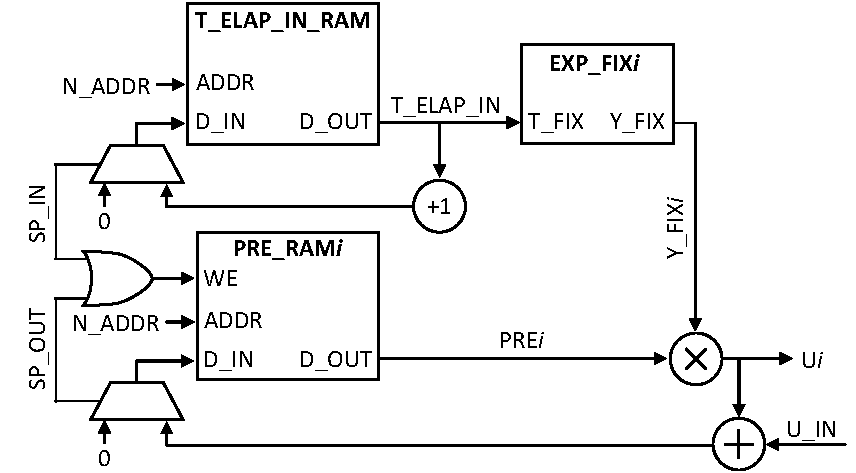
\includegraphics[width=3.4in]{fig6}
    \caption{\label{fig:fig6} Block diagram of the U$i$-evaluation circuit.}
\end{figure}
%%%%%%%%%%%%%%%%%%%%%%%%%%%

SRM$_\textrm{0}$ (Algorithm 2) for 512 neurons was implemented in a Xilinx Virtex-7 FPGA. 
Instructions 1 and 2 were realized using a U$i$ ($i$ = 1, 2) evaluation circuit (Fig. \ref{fig:fig6}).
This circuit is dedicated to each of U1 ($i$ = 1) and U2 ($i$ = 2). 
The circuit includes one EXP\textunderscore FIX$i$ module with time constant $\tau_\textrm{m}$ and $\tau_\textrm{s}$ for U1 and U2, respectively. 
The defining variables for each neuron are the time elapsed since the last input spike ($t$-$\hat{t_j}$) and pre-exponential factor, which are encoded as a 16-bit integer (T\textunderscore ELAP\textunderscore IN) and 12-bit fixed-point (Q4.8) value (PRE$i$), respectively.
One T\textunderscore ELAP\textunderscore IN and one PRE$i$ are dedicated to each of 512 neurons, which are separately stored in T\textunderscore ELAP\textunderscore IN\textunderscore RAM (512$\times$16b RAM) and PRE\textunderscore RAM$i$ (512$\times$12b RAM), respectively (Fig. \ref{fig:fig6}).  
The term $\tau_\textrm{m}$$\cdot$[($\tau_\textrm{m}$ - $\tau_\textrm{s}$)$\cdot$$\mathrm{\lvert}$$u_\textrm{hyp}$$\mathrm{\lvert}$]$^\textrm{-1}$$\cdot$$w_{ij}$ is encoded as a 12-bit fixed-point (Q4.8) value (U\textunderscore IN). 
On a given time step, the U$i$ values are evaluated sequentially for 512 neurons using an address pointer (N\textunderscore ADDR). Note that the U1 and U2 circuit can share T\textunderscore ELAP\textunderscore IN\textunderscore RAM because both use this variable in common. Subsequently, UM0 is evaluated from the U1 and U2 values following Instruction 3. 

%%%%%%%%%%%%%%%%%%%%%%%%%%%
\begin{figure}[t]\centering
    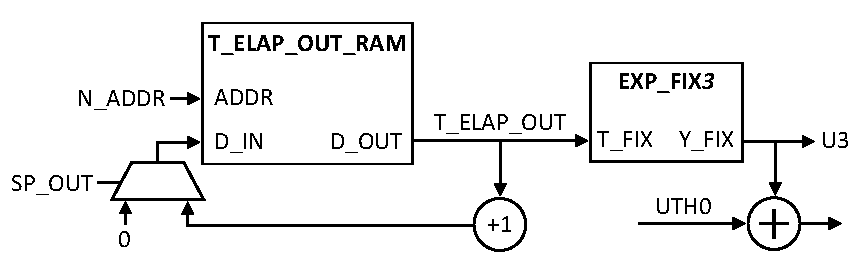
\includegraphics[width=3.4in]{fig7}
    \caption{\label{fig:fig7} Block diagram of the U3-evaluation and subsequent addition to UTH0 processes.}
\end{figure}
%%%%%%%%%%%%%%%%%%%%%%%%%%%

Fig. \ref{fig:fig7} shows a block diagram of U3 evaluation (following Instruction 4) and its subsequent addition to the normalized spiking threshold UTH0 for Instruction 5. 
The time elapsed since the last output spike ($t$-$\hat{t_i}$) is encoded as a 16-bit integer (T\textunderscore ELAP\textunderscore OUT). 
T\textunderscore ELAP\textunderscore OUT\textunderscore RAM (512$\times$16b RAM) stores T\textunderscore ELAP\textunderscore OUT for all 512 neurons. 
Similarly, the circuit includes one EXP\textunderscore FIX module (EXP\textunderscore FIX3).
The output (U3+UTH0) is compared with UM0 to generate a spike (SP\textunderscore OUT = 1) when larger than UM0. 
All signals used in this implementation and their formats are summarized in Table \ref{tab:tab2}.

The block diagrams in Figs \ref{fig:fig6} and \ref{fig:fig7} were implemented in an FPGA to build 512 SRM$_\textrm{0}$ neurons. 
Here, we consider two different architectures: (i) the use of three EXP\textunderscore FIX modules (one for each of the three U$i$-evaluation circuits ($i$ = 1, 2, and 3)) and (ii) two EXP\textunderscore FIX modules (one shared by the U1- and U3-evaluation circuits and one for the U2-evaluation circuit). 
The former and latter are referred to as the Three-EXP\textunderscore FIX and Two-EXP\textunderscore FIX architectures, respectively. 
The U1- and U3-evaluation circuits can share the same EXP\textunderscore FIX module because SRM$_\textrm{0}$ assumes the same time constant in the kernels $\eta$ and $\epsilon_\textrm{1}$ as shown in Eqs. \eqref{equ:equ14} and \eqref{equ:equ15}, respectively. 
This way saves hardware resources, but at the cost of an additional latency in calculation due to the time-multiplexing.

%%%%%%%%%%%%%%%%%%%%%%%%%%%
\begin{table*}[tbh]\centering
\caption{\label{tab:tab2} Signals used in SRM$_\textrm{0}$ implementation}
\renewcommand{\arraystretch}{1.25} 
\begin{threeparttable}\small
\begin{tabular}[ht]{p{2.5cm}p{8cm}p{3cm}l}\toprule \toprule
    \textbf{Signal name} 
        &\textbf{Description} 
        &\textbf{Data format} 
        &\textbf{Size}\\\midrule
    N\textunderscore ADDR
        &Neuron address 
        &Integer &8 bits\\
    EN  &Enable signal &Boolean &1 bit\\
    SEL &Select signal &Boolean &1 bit \\
    \multirow{2}{2.5cm}{U$i$} 
        &U1 ($i$ = 1) and U2 ($i$ = 2)  &Fixed-point (Q4.8) &12 bits \\
        &U3 ($i$ = 3)                   &Fixed-point (Q12)  &12 bits \\
    PRE$i$ 
        &Pre-exponential factor for U1 ($i$ = 1) and U2 ($i$ = 2)
        &Fixed-point (Q4.8) &12 bits \\
    T\textunderscore ELAP\textunderscore IN
        &Time elapsed since the last input spike
        &Integer &16 bits \\
    T\textunderscore ELAP\textunderscore OUT
        &Time elapsed since the last output spike
        &Integer &16 bits \\          
    Y\textunderscore FIX 
        &Output of EXP\textunderscore FIX 
        &Fixed-point (Q16) &16 bits\\
    U\textunderscore IN
        &Increase in U$i$ upon an input spike 
        &Fixed-point (Q4.8) &12 bits \\
    UTH0      
        &Normalized threshold for spiking &Fixed-point (Q4.8) &12 bits\\
    SP\textunderscore IN
        &Input spike 
        &Boolean &1 bit \\
    SP\textunderscore OUT
        &Output spike 
        &Boolean &1 bit \\
\bottomrule \bottomrule
\end{tabular}
\end{threeparttable}
\end{table*}
%%%%%%%%%%%%%%%%%%%%%%%%%%%

%%%%%%%%%%%%%%%%%%%%%%%%%%%
\begin{figure*}[b]\centering
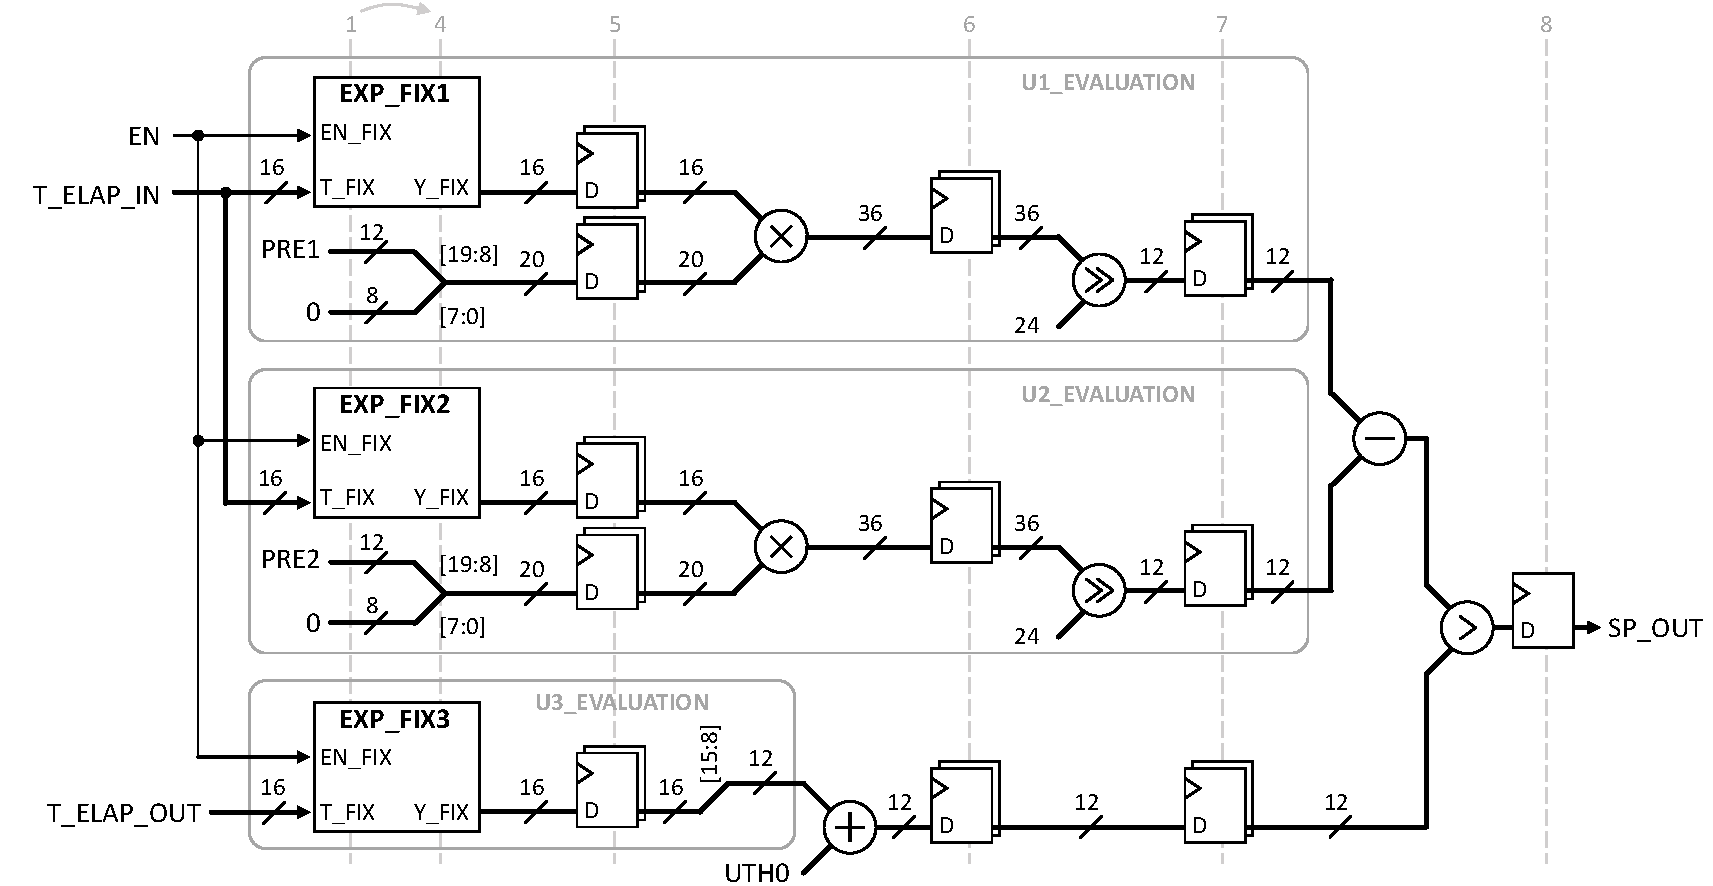
\includegraphics[width=7.1in]{fig8}
\caption{\label{fig:fig8} RTL diagram of the Three-EXP\textunderscore FIX architecture.}
\end{figure*}
%%%%%%%%%%%%%%%%%%%%%%%%%%%

An RTL diagram of the Three-EXP\textunderscore FIX architecture is shown in Fig. \ref{fig:fig8}. 
We used three EXP\textunderscore FIX modules, EXP\textunderscore FIX1, EXP\textunderscore FIX2, and EXP\textunderscore FIX3, for U1, U2, and U3 evaluation, respectively. 
As indicated in Table \ref{tab:tab2}, Y\textunderscore FIX is a 16-bit fixed-point value (all 16 bits are dedicated to its fractional part) while PRE$i$ ($i$ = 1 and 2) a 12-bit fixed-point value (Q4.8).
Before their multiplication, PRE$i$ is concatenated with an 8-bit zero register to change its format to Q4.16. 
This value is multiplied by Y\textunderscore FIX, and the resulting 36-bit value is rounded to a 12-bit fixed-point format (Q4.8) using a right-shift operator.
For the addition of U3 (16-bit fixed point (Q16)) to UTH0 (12-bit fixed point (Q4.8)), the last 8-bits of U3 is abandoned to yield a 12-bit fixed-point result (Q4.8), which is subsequently compared with U1 - U2 to determine SP\textunderscore OUT (0 or 1).
Because the implementation is fully-pipelined, each operation step takes one clock cycle. 
Therefore, it takes eight clock cycles (four cycles for the EFA and four cycles for the subsequent operations) for the circuit to determine SP\textunderscore OUT for each neuron (Fig. \ref{fig:fig8}).

%%%%%%%%%%%%%%%%%%%%%%%%%%%
\begin{figure*}[bth]\centering
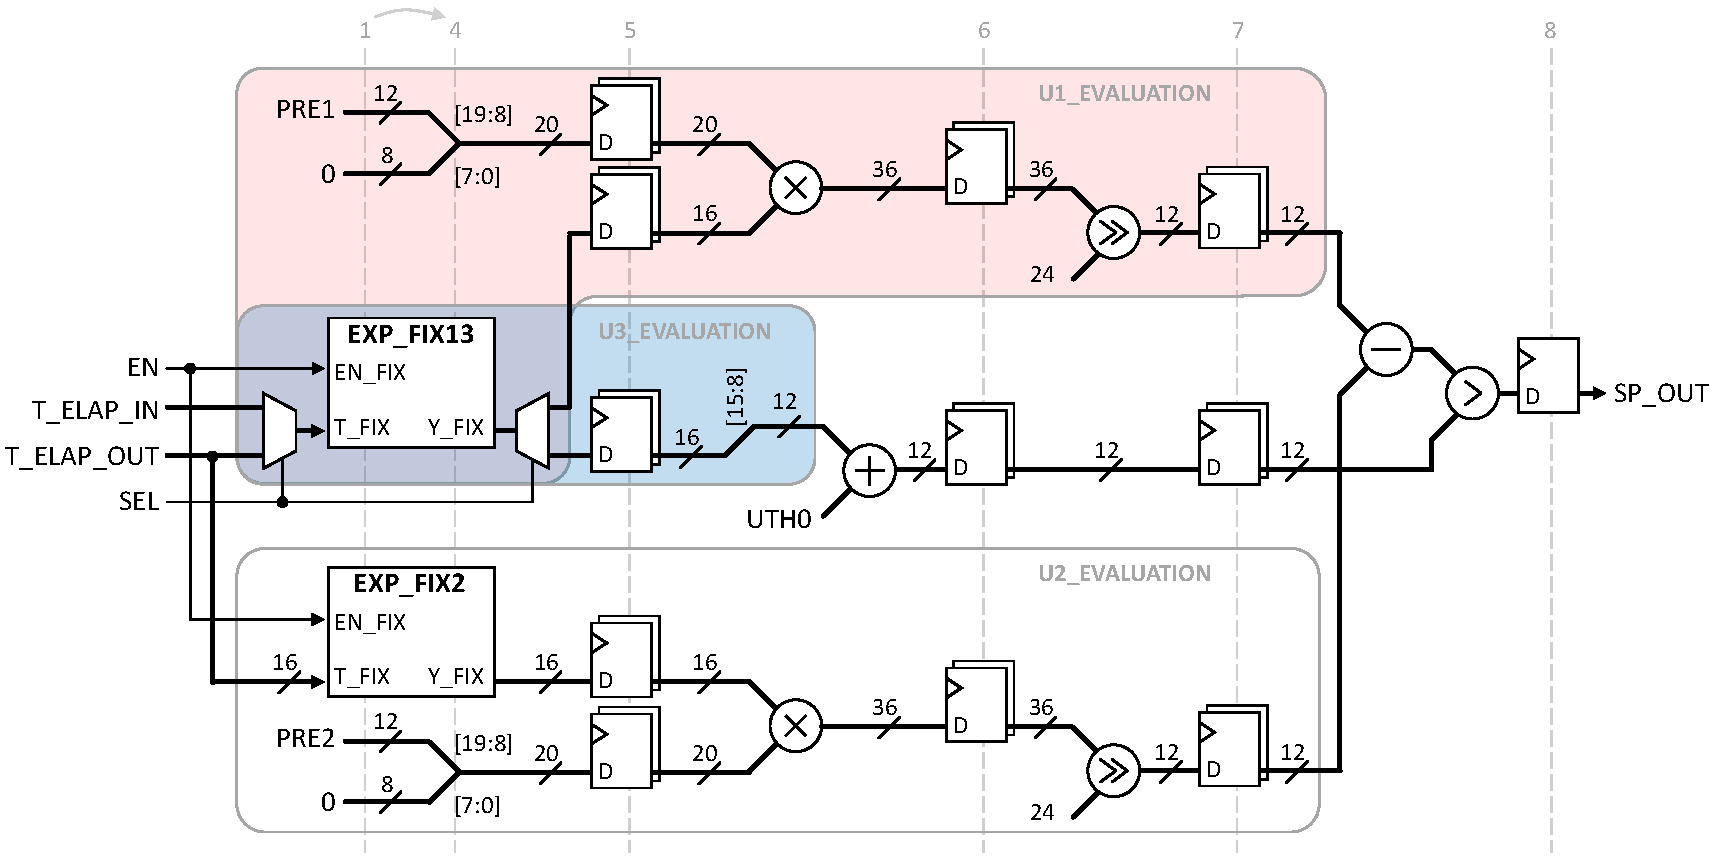
\includegraphics[width=7.1in]{fig9}
\caption{\label{fig:fig9} RTL diagram of the Two-EXP\textunderscore FIX architecture.}
\end{figure*}
%%%%%%%%%%%%%%%%%%%%%%%%%%%

For the Two-EXP\textunderscore FIX architecture with EXP\textunderscore FIX13 and EXP\textunderscore FIX2 modules, we used an additional clock (doubled clock speed) to prevent the additional latency due to sharing EXP\textunderscore FIX13. 
This is highlighted in the RTL diagram of the Two-EXP\textunderscore FIX architecture in Fig. \ref{fig:fig9}. 
Therefore, this architecture determines SP\textunderscore OUT with the same latency (eight clock cycles) as the Three-EXP\textunderscore FIX architecture. 
Given the use of two, rather than three, EXP\textunderscore FIX modules, it consumes fewer hardware resources than the Three-EXP\textunderscore FIX architecture as shown in Table \ref{tab:tab5}.

%%%%%%%%%%%%%%%%%%%%%%%%%%
\begin{table}[tb]\centering
\caption{\label{tab:tab4} Parameters used in SRM$_\textrm{0}$ implementation and simulation}
\renewcommand{\arraystretch}{1.2} 
\begin{threeparttable}\small
\begin{tabular}[ht]{lp{4.2cm}l} \toprule \toprule
    \textbf{Parameter} 
    &\textbf{Description} &\textbf{Value} \\\midrule
    ~~~$\Delta t$ 
        &Sampling precision &$2^\textrm{-12}$\\
    ~~~$u_\textrm{th}$ 
        &Spiking threshold&0.15\\
    ~~~$u_\textrm{hyp}$ 
        &Hyperpolarized membrane potential &-0.05\\
    ~~~$\tau_\textrm{m}$ 
        &Membrane potential decay time constant &0.04\\
    ~~~$\tau_\textrm{s}$ 
        &Synaptic current decay time constant &0.01\\
    ~~~$w_\textit{ij}$ &Synaptic weight &0.10\\
    ~~~$r$ &Input spike firing rate &[20.48, 102.4]\\
    ~~~\textit{T} &Period &16 s\\ \bottomrule \bottomrule
\end{tabular}
\end{threeparttable}
\end{table}
%%%%%%%%%%%%%%%%%%%%%%%%%%

\subsection{Performance evaluation}
\label{subsec:performance} 
Using the proposed SRM$_\textrm{0}$ circuits in an FPGA, we emulated neuronal response functions of 512 neurons with presynaptic Poisson spikes at different firing rates for a given period \textit{T} (=16 s). 
The neuronal parameters in Table \ref{tab:tab4} were used, which were shared by all 512 neurons. 
The firing rate of SRM$_\textrm{0}$ at a given presynaptic firing rate was measured by counting the spikes elicited from SRM$_\textrm{0}$ over the period \textit{T}.
The average firing rate on 30 trials was finally evaluated. 
The Two- and Three-EXP\textunderscore FIX architectures produced the same results.
To identify the accuracy of the proposed circuit, we compared the results with SRM$_\textrm{0}$ simulations using Algorithm 1 with real-valued neuronal parameters and variables (Fig. \ref{fig:fig10}).
The comparison identifies the high accuracy of emulation insomuch as the mean error is below 2\% for all presynaptic firing rates. 

%%%%%%%%%%%%%%%%%%%%%%%%%%%
\begin{figure}[!b]\centering
    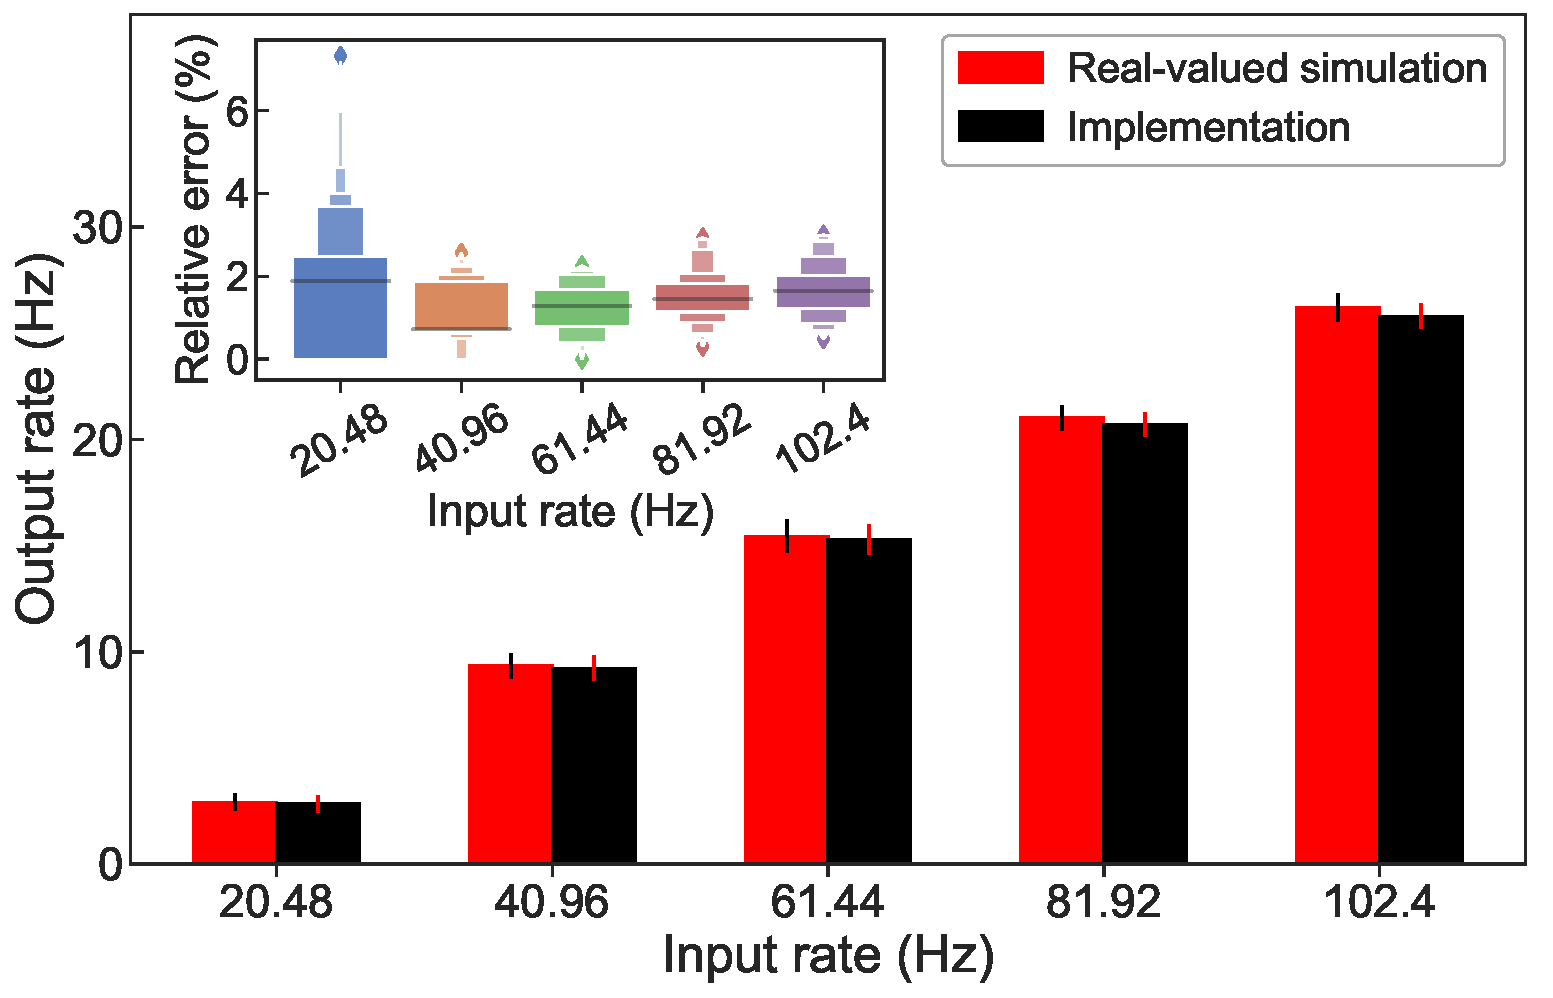
\includegraphics[width=3.49in]{fig10}
    \caption{\label{fig:fig10} Comparison between our SRM$_\textrm{0}$ implementation and simulation with real-valued parameters and variables in terms of output spike firing rates in response to input Poisson spikes. The inset shows a distribution of errors relative to the simulation results for each input rate.}
\end{figure}
%%%%%%%%%%%%%%%%%%%%%%%%%%%

We finally compared our neuronal circuit designs with related works in terms of hardware-resource consumption as shown in Table \ref{tab:tab5}. 
For a fair comparison, we estimated the memory usage solely for neuron implementation in the related works, which is shown in the rightmost column of Table \ref{tab:tab5}.
The implementation in \cite{caron2011fpga} proposed an LIF neuron-based SNN for pattern matching. 
The design consumes zero memory at the cost of the significant number of flip-flops (FFs) and LUTs as logic in use.
The implementation of the piecewise linear (PWL) model in \cite{soleimani2012biologically} uses approximately 18 \textendash~20 bit memory per neuron and a fewer FFs and LUTs than \cite{caron2011fpga}, but addresses merely 30 neurons.
Li \textit{et al}. \cite{li2012fpga} considered the silicon neuron model based on two variables (membrane potential and auxiliary variable representing the activity of ion channels) that are cross-coupled. 
The model is richer in dynamics than simple LIF neuron models and requires a significant amount of hardware resources including FFs, LUTs, DSP slices, and memory. 
Particularly, the memory usage attains 4,941 bit per neuron. 
Bonabi \textit{et al}. \cite{bonabi2014fpga} implemented the Hodgkin-Huxley (HH) model with large complexity in calculation by utilizing a number of FFs, LUTs, DSP slices, and memory. 
Particularly, the implementation uses 1,112 DSP slices.
Khoyratee \textit{et al}. \cite{khoyratee2019optimized} proposed an implementation of a modified HH model that is particularly tailored to digital circuits. 
Consequently, the implementation largely reduces the use of hardware resources compared with \cite{bonabi2014fpga} as shown in Table \ref{tab:tab5}.
Unfortunately, the memory usage is not available. 
Ambroise \textit{et al}. \cite{ambroise2013biorealistic} realized the Izhikevic model with two variables (membrane potential and auxiliary variable) using approximately 1,143b memory per neuron.


%%%%%%%%%%%%%%%%%%%%%%%%%%%%%%
\begin{table*}[t]\centering
\caption{\label{tab:tab5} comparison of our SRM$_\textrm{0}$ implementation with related works}
\renewcommand{\arraystretch}{1.2} 
\begin{threeparttable}\small
\begin{tabular}[ht]{lcccccc}\toprule\toprule
    &\multirow{2}{1.3cm}{\textbf{FF}} &\multirow{2}{1.3cm}{\textbf{LUTs\\as logic}} &\multirow{2}{1.3cm}{\textbf{DSP slices}} &\multirow{2}{1.5cm}{\textbf{Neuron of\\number, \textit{N}}} &\multirow{2}{3.5cm}{\textbf{Memory (type)}} &\multirow{2}{1.7cm}{\textbf{Memory per neuron$^\dagger$}}\\ 
    &&&&&&\\\midrule
    \multirow{2}{4cm}{\textbf{LIF neuron model} \\(Caron \textit{et al}. \cite{caron2011fpga})} 
        &\multirow{2}{1.3cm}{12,058$^\dagger$} 
        &\multirow{2}{1.3cm}{19,531$^\dagger$} 
        &\multirow{2}{1.3cm}{$-^\dagger$} 
        &\multirow{2}{1.5cm}{648$^\dagger$} 
        &\multirow{2}{3.5cm}{0$^\dagger$ (BRAM$^\ddagger$)} 
        &\multirow{2}{1.5cm}{0$^\dagger$}\\ 
    &&&&&&\\
    \multirow{2}{4cm}{\textbf{PWL model} \\(Soleimani \textit{et al}. \cite{soleimani2012biologically})}
        &\multirow{2}{1.3cm}{374$-$493} 
        &\multirow{2}{1.3cm}{453$-$617} 
        &\multirow{2}{1.3cm}{$-$}  
        &\multirow{2}{1.5cm}{30} 
        &\multirow{2}{3.5cm}{150$-$158 Byte ($-$)}
        &\multirow{2}{1.7cm}{18b$-$20b$^\pounds$}\\
    &&&&&&\\
    \multirow{2}{4cm}{\textbf{Spiking silicon neuron model} \\(Li~\textit{et al}. \cite{li2012fpga})} 
        &\multirow{2}{1.3cm}{14,198} 
        &\multirow{2}{1.3cm}{18,556} 
        &\multirow{2}{1.3cm}{48}   
        &\multirow{2}{1.5cm}{256} 
        &\multirow{2}{3.5cm}{73$\times$18Kb (BRAM$^\ddagger$)} 
        &\multirow{2}{1.7cm}{4,941b$^\pounds$} \\
    &&&&&&\\
    \multirow{2}{4cm}{\textbf{Hodgkin-Huxley model}\\ (Bonabi \textit{et al}. \cite{bonabi2014fpga})} 
        &\multirow{2}{1.3cm}{50,228} 
        &\multirow{2}{1.3cm}{86,032} 
        &\multirow{2}{1.3cm}{1,112} 
        &\multirow{2}{1.5cm}{150} 
        &\multirow{2}{3.5cm}{15$\times$18Kb (BRAM$^\ddagger$)} 
        &\multirow{2}{1.7cm}{1,568b$^\pounds$} \\
    &&&&&&\\
    \multirow{2}{4cm}{\textbf{Hodgkin-Huxley model} \\(Khoyratee \textit{et al}. \cite{khoyratee2019optimized})} 
        &\multirow{2}{1.3cm}{1,552} 
        &\multirow{2}{1.3cm}{4,735} 
        &\multirow{2}{1.3cm}{16}   
        &\multirow{2}{1.5cm}{1,034} 
        &\multirow{2}{3.5cm}{$-$} 
        &\multirow{2}{1.7cm}{$-$} \\
    &&&&&&\\
    \multirow{2}{4cm}{\textbf{Izhikevich model} \\(Ambroise \textit{et al}. \cite{ambroise2013biorealistic})} 
        &\multirow{2}{1.3cm}{970} 
        &\multirow{2}{1.5cm}{1,598} 
        &\multirow{2}{1.3cm}{$-$}   
        &\multirow{2}{1.5cm}{117} 
        &\multirow{2}{3.5cm}{144Kb ($-$)} 
        &\multirow{2}{1.7cm}{1,143b$^\pounds$} \\
    &&&&&&\\
    \multirow{4}{4cm}{\textbf{Simplified spike-response} \\\textbf{model} (This work) 
        \\~~~$\cdot$ Two-EXP\textunderscore FIX 
        \\~~~$\cdot$ Three-EXP\textunderscore FIX}
        &\multirow{4}{1.3cm}{\\~\\296 \\278} 
        &\multirow{4}{1.3cm}{\\~\\314 \\335} 
        &\multirow{4}{1.3cm}{\\~\\4 \\5}   
        &\multirow{4}{1.5cm}{\\~\\512 \\512} 
        &\multirow{4}{3.5cm}{\\~\\1,003$\times$64b (Dist. RAM$^\S$) \\1,179$\times$64b (Dist. RAM$^\S$)} 
        &\multirow{4}{1.7cm}{\\~\\125b$^\pounds$ \\147b$^\pounds$} \\
    &&&&&&\\ &&&&&&\\ &&&&&&\\
\bottomrule \bottomrule
\end{tabular}
\begin{tablenotes}\small
\item[$\dagger$] This is the number of hardware units dedicated to neuron implementation;
\item[$\ddagger$]: Block RAM
\item[$\pounds$] $\frac{N}{2}\times\frac{N}{2}$ fully-connected network with 3-bit weights were assumed.
\item[$\S$]: Distributed RAM
\end{tablenotes}
\end{threeparttable}
\end{table*}
%%%%%%%%%%%%%%%%%%%%%%%%%%%%

Our implementation of 512 SRM$_\textrm{0}$ neurons features the highly efficient use of hardware resources compared with the aforementioned works. 
Particularly, the Two-EXP\textunderscore FIX architecture uses 1,003$\times$64b memory for 512 neurons, i.e., 125b per neuron. 
Considering the memory dedicated to the EXP\textunderscore FIX modules (\textit{M}$_\textrm{EXP\textunderscore FIX}$ = 2$\times$11,264b) shared among all neurons, the memory usage per neuron largely decreases with the number of neurons implemented. 
The total usage of memory for \textit{N} neurons \textit{M}$_\textrm{tot}$ is given by \textit{M}$_\textrm{tot}$ = \textit{M}$_\textrm{EXP\textunderscore FIX}$ + \textit{M}$_\textrm{n}$$\cdot$\textit{N}, where \textit{M}$_\textrm{n}$ is approximately 80b.  
Therefore, the memory usage per neuron is \textit{M}$_\textrm{EXP\textunderscore FIX}$$\mathbin{/}$\textit{N} + \textit{M}$_\textrm{n}$. 
For instance, this value decreases down to only 82.2b$\mathbin{/}$neuron when implementing 4,000 neurons. 



\section{Conclusion}\label{sec:con}
We proposed the TS-EFA method and its implementation in an FPGA, which forms the highly efficient basis of SRM$_\textrm{0}$ implementation. 
TS-EFA highlights high-precision and low-latency EFAs with a fewer hardware resources (LUTs as logic and memory) than related works.
The implementation of SRM$_\textrm{0}$ using TS-EFA leverages its high-precision and low-latency approximation with high-efficiency in hardware consumption. 
To this end, we first proposed an algorithm for SRM$_\textrm{0}$ using three sub-kernels, each is given by a simple exponential function. 
Subsequently, the algorithm was modified to render it suitable for its implementation using the TS-EFA method. 
The results confirm (i) high-precision simulations of neuronal response functions compared with the SRM$_\textrm{0}$ based one real-valued variables and parameters (average error rate was below 2\%), (ii) low latency (eight clock cycles), and (iii) efficient usage of hardware resources, particularly, memory usage per neuron ($\sim$125b).      


%\setcounter{table}{0}
%\renewcommand{\thetable}{A\arabic{table}}

%\appendices
%\section{}

%%%%%%%%%%%%%%%%%%%%%%%%%%

\section*{Acknowledgement}
This work was supported by the research grant of the National Research Foundation of Korea under Grant NRF-2019R1C1C1009810.

\bibliography{Bib.bib}

\begin{IEEEbiography}[{
\includegraphics[width=1in,height=1.3in,clip]{Jeeson_Kim}}]{Jeeson Kim} received the B.Eng. degree in semiconductor systems engineering from the Catholic University of Korea, South Korea, in 2011, and the M.Eng. and Ph.D. degrees in electrical and electronic engineering from RMIT University, Australia, in 2014 and 2019, respectively. She is currently a Postdoctoral Scholar with Hanyang University, South Korea. Her research interests include nano-enabled hardware security, low-power solutions for cyber-physical systems, and analog and digital designs for neuromorphic systems.
\end{IEEEbiography}

\begin{IEEEbiography}[{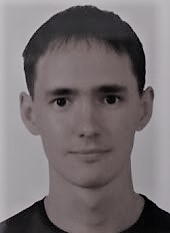
\includegraphics[width=1in,height=1.3in,clip]{Vladi_K}}]{Vladimir Kornijcuk} received the B.S. degree in Telecommunication Physics and electronics from Vilnius University, Vilnius, Lithuania and the M.S. degree in Materials Science and Engineering from Seoul National University of Science and Technology, Seoul, Republic of Korea. He received his PhD degree in Nano and Information Technology at the University of Science and Technology, Seoul, Republic of Korea. He is current a postdoctoral scholar at Hanyang Univeristy, Republic of Korea. His current research interest includes digital neuromorphic processor design.
\end{IEEEbiography}

\begin{IEEEbiography}[{
\includegraphics[width=1in,height=1.3in,clip]{Changmin_Ye}}]{ChangMin Ye}
received his B.Eng. degree in Materials Science and Engineering from the Hanyang University, Seoul, South Korea, in 2020. He is currently in the master\rq{}s course in Materials Science and Engineering with Hanyang University, Seoul. Since 2019, he has been focusing on learning digital neuromorphic processor design.
\end{IEEEbiography}

\begin{IEEEbiography}[{
\includegraphics[width=1in,height=1.3in,clip]{Dooseok_Jeong}}]{Doo Seok Jeong} is an Associate Professor at Hanyang University, Republic of Korea. He received his BE and ME in Materials Science from Seoul National University in 2002 and 2005, respectively. He received his PhD degree in Materials Science from RWTH Aachen, Germany in 2008. He was with the Korea Institute of Science and Technology from 2008 to 2018. His research interest includes spiking neural networks for sequence learning and future prediction. Learning algorithms, spiking neural network design, and digital neuromorphic processor design are his current research focus.
\end{IEEEbiography}

\end{document}